\chapter{Scanner}\label{sec:scanner}
When it comes to automatically generating textured 3D models from real-world objects, photogrammetry is the obvious choice.
Broadly speaking, it is the process of obtaining information about the objects using their images (in our case, the model and the texture).
It can be done cheaply, since it only requires high-quality images of the modelled object, which can be obtained using either a~digital camera, or any recently released mobile phone (further discussed in section \ref{sec:camsettings}).

Besides photogrammetry, another option for creating 3D models is laser scanning.
This was not a~viable option due to the high price, because products that could be used (such as Revopoint POP, XYZ 1.0 Pro or the Creality 3D Scanner) cost upwards of $10\ 000$ CZK ($420$ USD), which is non-trivial considering only a~potential quality improvement.
However, since a~number of the aforementioned programs support laser scanning out of the box, the photogrammetry approach could be combined with laser scanning and thus enjoy the advantages of both.

\section{Feature-based photogrammetry}
Because the problem of creating 3D models from images is difficult and involves a~lot of steps and specialized algorithms, many open-source and proprietary programs have been developed to simplify this task.

This thesis uses the Agisoft Metashape photogrammetry software \cite{metashape}.
While there are other suitable photogrammetry programs such as Meshroom (free), 3DF Zephyr (commercial) and COLMAP (free), Metashape was chosen for the following reasons:
\begin{itemize}
	\item It created the highest-quality models out of the tested programs, given a~representative sample of the hold images, which consisted of a~foothold, two regular holds and a~dual texture hold.
	\item It includes a~well-documented Python API, along with a~good GUI.
\end{itemize}

Since it is closed-source, there is no easy way to determine the exact algorithms used.
However, a~forum statement from the lead developer Dimitry Seymonov~\cite{metashapeForumPost}, with addition of license files for various open-source projects included with Metashape, give a~good overview of the general methods used.

Starting with a~set of images and ending with a~textured model, the process can be split into the following parts:

\begin{enumerate}
	\item \textbf{feature extraction:} for each image, find features that are stable under linear and affine transformations, viewpoint change and illumination
	\item \textbf{feature matching:} find matching features across multiple images
	\item \textbf{bundle adjustment:} find the approximate positions of the camera and the matched features (obtaining ``structure from motion'' data)
	\item \textbf{dense point cloud generation:} obtain additional features (along with their normals) for higher model quality
	\item \textbf{surface reconstruction:} reconstruct the surface of the model
	\item \textbf{texturing:} map a~texture from the images onto the model
\end{enumerate}

The following sections aim to cover each of these in part.

\subsection{Feature extraction} \label{ch:fext}
The image features are extracted using the Scale Invariant Feature Transform (SIFT) method described in \citet{lowe1999object,lowe2004distinctive}.
Each of the features is a~vector describing some properties of a~pixel of the image and should be invariant or partially invariant to linear and affine transformations, illuminance change and 3D transformations.

To find such vectors, a~Gaussian scale-space is used.
Formally, a~scale-space for a~given 2D image $I(x, y)$ is defined as a~function
\begin{equation} L(x, y, \sigma) = G(x, y, \sigma) * I(x, y) \end{equation}

The $*$ symbol is a~convolution of the two functions in $x$ and $y$, and $G$ is the Gaussian function
\begin{equation}G(x, y, \sigma) = \frac{1}{2\pi \sigma^2}\ \mathrm{e}^{-(x^2 + y^2) / 2\sigma^2}\end{equation}

This operation is applied twice to image $I$ with $\sigma = \sqrt{2}$, yielding images $I_{1,1}, I_{2,1}$, the difference of which yields the image $G_1$ (see figure \ref{fig:gaussexample}).
After this, the image $I_{2,1}$ is downscaled by a~certain factor (the original method uses $1.5$ with bilinear interpolation) and the process is repeated, yielding $I_{1,2}, I_{2,2}$ and $G_2$, respectively.

\begin{figure}
	\centering
	\includegraphics[width=\columnwidth]{images/gauss/gauss-smol.jpg}
	\caption{An example of the convolution and difference applied to a~hold image. Generated using Python and the NumPy, SciPy and the Pillow libraries.}
	\label{fig:gaussexample}
\end{figure}

To find the vectors, the local minima and maxima of the pixels of $G_1$ (compared to the 8 neighbouring pixels) are examined --- if they are also minima/maxima in~$G_2$ (accounting for the downscaling), they are selected as features.
The intuitive idea behind this approach is to suppress the finer details of the image, since each of the main features of the original image should be present in the ``coarse/blurred'' version \cite{scalespace}.

To calculate the vectors for the selected pixels, the vector's magnitude $M(x,y)$ and orientation $R(x,y)$ is determined using their neighbouring points via the following formulas:
\begin{align}
	M(x,y) &= \sqrt{\left(I_{1,1}(x, y) - I_{1,1}(x + 1, y)\right)^2 + \left(I_{1,1}(x,y) - I_{1,1}(x, y + 1)\right)^2} \\[0.7em]
	R(x,y) &= \mathrm{atan2} \left(I_{1,1}(x, y) - I_{1,1}(x + 1, y), I_{1,1}(x,y) - I_{1,1}(x, y + 1)\right)
\end{align}

The $\mathrm{atan2(x, y)}$ function used returns the angle between the $x$ axis and the point $(x, y)$.
It is a more general version of the $\mathrm{atan(y/x)}$ function, which doesn't distinguish points like $(-x, -y)$ and $(x, y)$ (since only their ratio is used).

For the vectors to be invariant to orientation and contrast changes, a~canonical representation is calculated from their local image gradients.

A note to be made is that SIFT can be utilized in other feature-matching problems such as stitching panoramas and finding objects in images, which could potentially be used to locate hold models.

\subsection{Feature matching}
Once the canonical representations of the vectors have been calculated, the images are examined pairwise.
For each feature in one image, the nearest neighbour (in terms of the vector distance in a~suitable norm) is found in the other.
To filter out features that only appear in one of the images, a~limit is imposed on the ratio of the distances between the closest and the second closest neighbour --- intuitively, good features should have only one matching candidate.

Since the number of features to match can be quite large and no efficient exact algorithm exists for the problem of finding the nearest neighbour, an approximate algorithm called best-bin-first is used \cite{beis1997shape}.
This algorithm returns the nearest neighbour with a~high probability, otherwise returning a~close one.
It internally uses a~$k$-d tree to partition the space into bins of the feature vectors, which it then searches in an efficient way.

\subsection{Bundle adjustment}
After the features have been determined and matched across the images, the next step is to simultaneously calculate their position in the 3D space and also the positions of the cameras.
This is referred to as the bundle adjustment problem~\cite{triggs1999bundle}, the name referring to bundles of rays from the predicted positions of the points going into the cameras.

Formally, we can model the scene by $n$ vectors of 3D points $\mathbf{X}_{i \in [n]}$ (sometimes called a~sparse point cloud), taken from $m$ cameras with parameters given by vectors $\mathbf{P}_{j \in [m]}$ (position, focal length, etc.).
The features can then be seen as observations $\overline{\bm{x}}_{ij}$ of point $i$ from camera $j$.

Let's now assume that we have a~function $\bm{x}(\mathbf{X}_i, \mathbf{P}_j)$ that, given the feature position $\mathbf{X}_i$ and camera parameters $\mathbf{P}_j$, models the calculated observation position $\mathbf{x}_{i, j}$.
Given this function, the bundle adjustment problem can be formulated as a~minimization problem of the function \begin{equation} \Delta x_{i, j} (\mathbf{X}_i, \mathbf{M}_j) = \overline{\bm{x}}_{ij} - \bm{x}(\mathbf{X}_i, \mathbf{P}_j) \end{equation} over the observed features, with an appropriate cost function. For estimation using nonlinear least squares, the cost function to minimize is the weighted sum of squared error, formulated as 
\begin{equation} \frac{1}{2} \sum_{i,j} \Delta x_{i, j} (\mathbf{X}_i, \mathbf{M}_j)^T W_{i,j} \Delta x_{i, j} (\mathbf{X}_i, \mathbf{M}_j) \end{equation}
where each $W_i$ is a~symmetric positive definite matrix indicating the weight of the vector, chosen to be approximately the inverse measured covariance of $\overline{\bm{x}}_{ij}$ (to account for the accuracy of measured feature points).

\begin{figure}[h]
	\centering
	\subfloat[Sparse point cloud.]{{\includegraphics[height=5.3cm]{images/pointclouds/sparse.png} }}%
	\hfill
	\subfloat[Dense point cloud.]{{\includegraphics[height=5.3cm]{images/pointclouds/dense.png} }}%
	\caption{Sparse and dense point cloud comparison on a~sample hold, generated using Agisoft Metashape.}%
\end{figure}

\subsection{Dense point cloud generation}
Since the feature matching step generates a~small number of features compared to what should be used to generate a~``high-quality'' mesh, additional feature points have to be generated.
The approach is based on generating depth-maps (grayscale images indicating the distance of each pixel from the camera) for each image and merging them together \cite{shen2013accurate}.

\subsubsection{Stereo pair selection}
First, each (target) image is paired with another (reference) image to generate its depth-map.
The reference image should view the object from a~similar direction but a~different angle that is not too close (\ang{5}) and too far (\ang{60}).
The camera centers should additionally be between $2 \overline{d}$ and $0.05 \overline{d}$, where $\overline{d}$ is the median of the distances between the images within the viewing angle.

The reference image is selected as the one minimizing the product of the viewing angle and the camera center distance, while the others (sorted and limited to 10) are considered the image neighbourhood $N_i$.

\subsubsection{Depth-map computation}
The core of the computation is based on the PatchMatch algorithm \cite{barnes2009PAR}.

A random 3D point, along with a~normal (forming a~plane), is assigned to each of the pixels of all images, such that they are in the viewing ray of their camera.
For each of the pixels, a~square ``patch'' centered on the pixel is placed on the image.
Then, for each pixel in it (across the reference image), a~matching cost is calculated (how well the point corresponding to the pixel fits with the others).
This cost is then iteratively improved either by moving the point to the plane of one of its neighbours, or by randomly changing it.

\subsubsection{Depth-map refinement}
To make the depth of the common areas consistent, each pixel of the depth-maps is considered --- if its corresponding point is close to its position in the neighbouring images $N_i$ (when projecting it onto the neighbouring image and then back using the neighbouring image depth-map), it is retained; otherwise it is removed from the depth-map.

\subsubsection{Depth-map merging}
The calculated depth-maps for each image are merged by taking their pixels' points and combining them to form the resulting dense point cloud.
To prevent duplication, the depth-maps are filtered by comparing their overlap with their neighbouring images.

\subsection{Surface reconstruction}
For surface reconstruction, the Poisson surface reconstruction algorithm \cite{kazhdan2006poisson} is used.
It takes points in 3D space and their normals (oriented towards the object), and constructs a~function that represents the surface.

It does this by first computing a~piecewise indicator function $\chi$ that is $0$ outside of the model and $1$ inside. The gradient of this indicator function (when convolved with a~suitable smoothing filter) is a~vector field, whose values near the surface are the point normals.

The problem can thus be formulated as a~minimization problem in terms of the difference between observed normals as a~vector field $\vec{V}$, and the indicator function gradient (denoted as $\nabla$):
\begin{equation} \min_\chi \Vert \nabla \chi - \vec{V} \Vert \end{equation}

Since we only have a~set of points and their normals, the difference in vector fields is approximated by a discrete sum.
Least squares are again used to find the solution (using the euclidean norm for the minimized vectors).

\subsection{Texturing}
All that is left is to create a~texture for the modeled object.
Since both the model and the camera position are known at this point, the images can be projected onto the faces in view (given that the face is pointed towards the camera).
Additional steps can be taken to normalize certain properties of the images, such as their brightness, contrast, etc.

\begin{figure}[b]
	\centering
	\subfloat[Textured view.]{{\includegraphics[height=2.3cm]{images/texture/texture.jpg} }}%
	\hfill
	\subfloat[Wireframe view.]{{\includegraphics[height=2.3cm]{images/texture/wireframe.jpg} }}%
	\caption{Model of a sample hold, generated using Agisoft Metashape.}%
\end{figure}

\section{Creating hold models}
Since a~regular climbing wall contains hundreds or even thousands of holds of varying sizes, it would be infeasible to model each of them manually.
It is therefore important to automate as many steps as possible so that the amount of manual work done is minimized.

It would be convenient if this could be done with the holds still on the wall, but this is difficult to accomplish for a~few reasons:
\begin{itemize}
	\item the scale and position of each hold would be difficult to infer,
	\item the hold boundary could not be clear (holds can be placed on top of each other, they can be touching side-by-side, etc.), and
	\item the quality of the models (texture and model-wise) might not be sufficient.
\end{itemize}

Having the holds off the wall, one way to automate the scanning is to construct a~turntable that turns the hold, with a~stationary camera taking the images from different angles.
If both the turntable and the camera are programmable, the time spent doing manual work would only include replacing one hold with another when the scanning is finished.

It would be unreasonable to expect the turntable to carry any hold, since larger structures can weigh tens of kilograms and measure more than a~meter.
However, both the carry weight and size should still be maximized.
Additionally, faster turntable rotation corresponds to quicker scanning and should thus also be maximized.

\subsection{Turntable design}
A three stepper-motor turntable (figure \ref{fig:turntable}) has been developed and 3D printed using the Fusion 360 CAD software \cite{fusion} and an Ender Pro 5 3D printer.
An Arduino board and A4988 motor controllers (figure \ref{fig:wiring}) are used for fine motor control.
The models, the code and a~short tutorial on the turntable construction are freely available at the Clis GitHub page \cite{clis}.

\begin{figure}[b!]
	% opravdu doufám, že tenhle kód nikdo číst nebude lmao
	\centering
	\subfloat[\centering Bottom part (side).]{{\includegraphics[height=3.6cm]{images/turntable/side.jpg} }}%
	\hfill
	\subfloat[\centering Bottom part (top).]{{\includegraphics[height=3.6cm]{images/turntable/bottom.jpg} }}%
	\hfill
	\subfloat[\centering Top part.]{{\includegraphics[height=3.6cm]{images/turntable/top.jpg} }}%
	\\
	\subfloat[\centering Bottom part (side).]{{\includegraphics[height=3.6cm]{images/realturntable/base2.jpg} }}%
	\hfill
	\subfloat[\centering Plexiglass (top).]{{\includegraphics[height=3.6cm]{images/realturntable/top2.jpg} }}%
	\hfill
	\hspace{1.2em}
	\subfloat[\centering Plexiglass (bottom), connected to the top part.]{{\includegraphics[height=3.6cm]{images/realturntable/top1.jpg} }}%
	\caption{Parts of the model of the turntable, generated using Fusion 360 (top row) and photographed using the Nikon z50 DLSR (bottom row). }%
	\label{fig:turntable}
\end{figure}

Communication with the Arduino is implemented via the USB port.
The protocol is simple --- the Arduino listens on the serial port until it receives a~string.
After reading it, it interprets it as integer and turns the corresponding number of degrees.
After the turn, it writes this number back to the serial port and again starts listening for another string.

The gphoto2 \cite{gphoto2} library is used to control the camera.
Its API can capture images, focus the camera and also interact with the camera file system.
All of the images were taken using Nikon z50 with a~Nikkor 18-55mm f/3.5--5.6 lens.

To minimize the amount of friction, the only points of contact between the top and bottom part of the turntable are 7 bearings (6 placed in a~circular pattern and 1 placed in the middle).
Additionally, gears mounted to the motors turn the top of the turntable, achieving a~$90/12 = 7.5$ reduction.
This allows the turntable to handle objects of up to \SI{8}{\kilo\gram}, with heavier objects requiring manual turning.

\begin{figure}[t]
	\centering
	\includesvg[width=\columnwidth]{images/wiring.svg}
	\caption{The wiring diagram of the turntable, created using Fritzing \cite{fritzing}.}
	\label{fig:wiring}
\end{figure}

The top area is connected to a~$\SI{50}{\centi\meter} \times \SI{50}{\centi\meter}$ plexiglass with a~marked center and 4 markers (to infer scale and position, see section \ref{sec:markersss}). This means that any hold that can fit on the plexiglass (and possibly extend beyond it, as long as it is not blocking the markers) can be scanned automatically.

The resulting workflow can model a~single hold in $1$ minute of scanning (varying depending on the lighting conditions and the number of photos, the default being $12$) and additional $4$ minutes of processing.\footnote{Computed using Metashape on Linux with AMD Ryzen 7 1700 and AMD Radeon RX 5500.}

\subsection{Scale and position inference}\label{sec:markersss}
The hold size and position (in local coordinates) needs to correspond to its real counterpart.
To do this automatically, markers are placed around it --- since their position in space is known (measured in advance), it can be used to infer the correct scale and position of the entire model.

The type of the markers supported by Metashape is based on \citet{schneider19913,borisPatent}.
Each circular target contains an inner and outer circle, the inner being used for locating the marker in the image and the outer for encoding the marker data.

The exact number of stored bits depends on the size of the marker, most common being $12$ and $14$, respectively.
The $0$ bits correspond to white segments and $1$ to black ones.
For decoding correctness and robustness, the following constraints are additionally imposed on the targets:

\begin{itemize}
	\item the targets must be rotationally invariant
	\item the first bit is a~parity bit ($0$ for even, $1$ for odd)
	\item there must exist an opposing pair of $1$ bits
\end{itemize}

After the positions of the markers are determined in 3D space (they are a~special type of feature described in section \ref{ch:fext} that uses a~different algorithm to be located across the images), it is just a~matter of simple linear algebra to transform the model appropriately.

\begin{figure}[t]
	\centering
	\includesvg[width=0.9\columnwidth]{images/targets.svg}
	\caption{The 18th 14-bit marker (left) and its corresponding binary value (right). Grey denotes an opposing pair of $1$ bits, blue denotes the parity bit. See \cite{targetsPost} for a comprehensive list of all markers, along with code that generates all valid marker binary values.}
\end{figure}

\subsection{Environment setup}
Two LED lights, mounted on adjustable stands and covered with baking paper (for light diffusion) were used to achieve good lighting conditions.
A large black cloth was used as the background to reduce false image features.

The entire setup can be carried in a~backpacking pack,\footnote{Excluding the plexiglass, which is inflexible and the camera, which is fragile.} making it portable.
Additionally, all of the setup components (excluding the camera) can be purchased for under $4000$ CZK ($180$ USD), making it affordable.

\begin{figure}
	\centering
	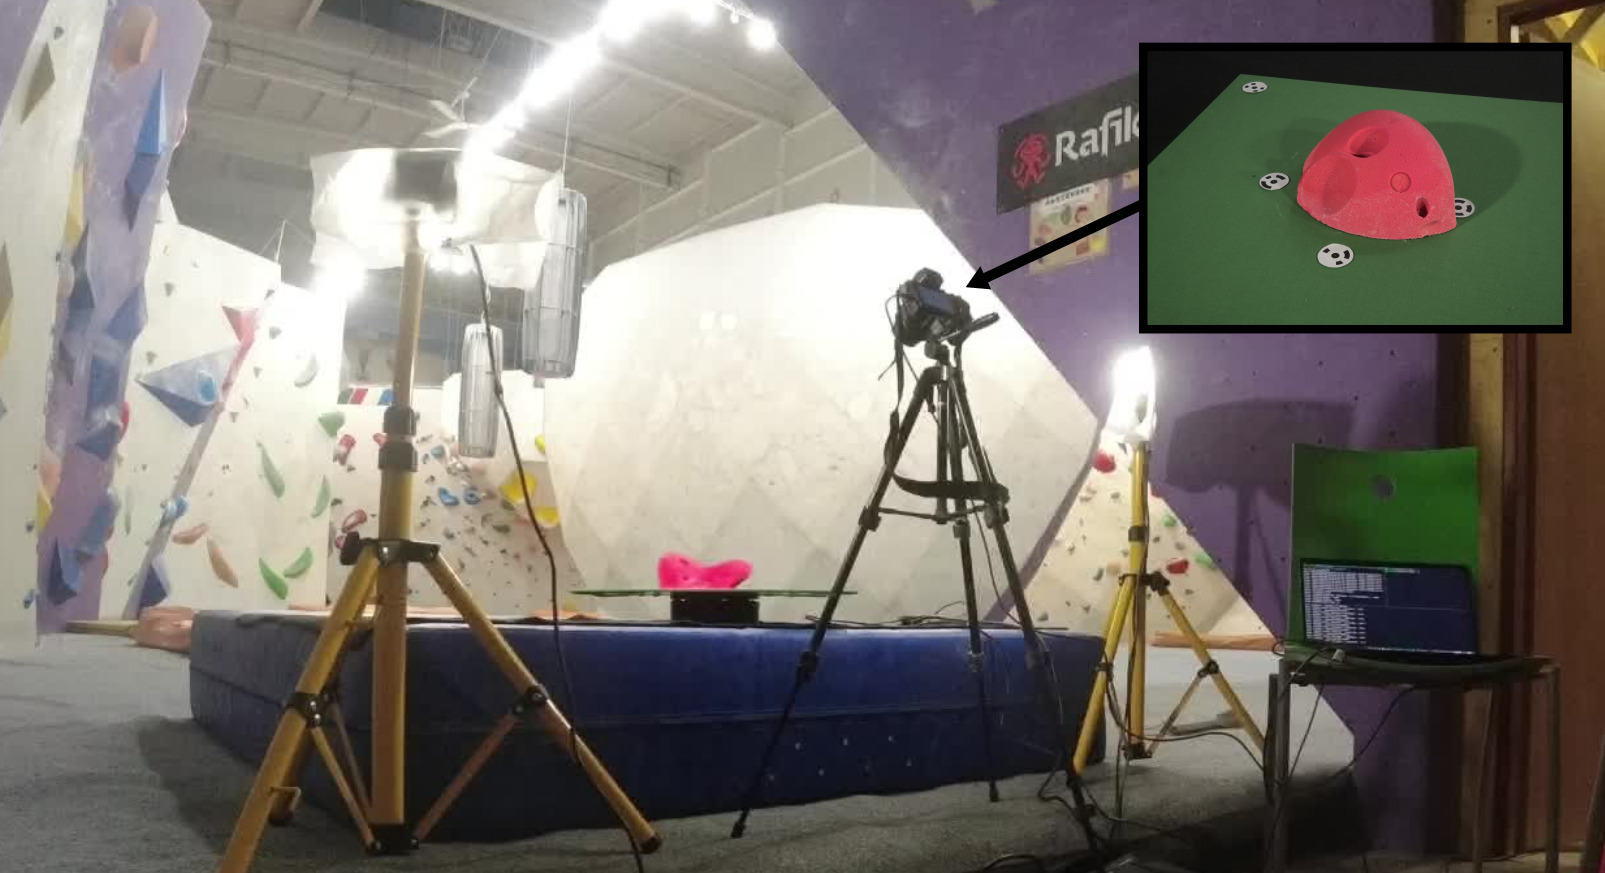
\includegraphics[width=\columnwidth]{images/setup/setup.jpg}
	\caption{An image of the setup during scanning, including the taken image.}
	\label{fig:setup}
\end{figure}

\subsection{Camera settings}\label{sec:camsettings}
Photogrammetry works best with sharp, high-resolution images with the least amount of noise possible.
To achieve this, the following settings were used to take all of the images:
\begin{itemize}
	\item resolution: $5600 \times 3728$
	\item ISO sensitivity: 320 --- lower sensitivity generally means less image noise
	\item aperture: 22 --- higher aperture widens the focal plane, which results in the entire scanned object being in focus and thus reducing blur
	\item exposure time: apx. $\SI{1.5}{\second}$ --- calculated from the sensitivity and the aperture for the image to have the correct brightness
\end{itemize}

The settings could only be used since the camera is static and the hold doesn't move while taking the image, otherwise the exposure time would be too high.

\subsection{Image masking}
The photogrammetry software expects the images to be viewed from various angles.
This poses a~problem for the turntable setup, since the background might not be perfectly dark and thus create false image features.
Fortunately, the contrast between the scanned area and the background is large enough to automatically construct a~mask to filter the background out.
This is done using OpenCV \cite{opencv} (as seen in figure \ref{fig:mask}) by
\begin{enumerate}
	\item converting the image to grayscale,
	\item generating a~binary image using a~threshold on the pixel brightness,
	\item applying a~contour-generating algorithm \cite{suzuki1985topological} on the image and finally
	\item using the largest (flood-filled) contour as the image mask.
\end{enumerate}

\begin{figure}[h]
	% opravdu doufám, že tenhle kód nikdo číst nebude lmao
	\centering
	\subfloat[\centering Original.]{{\includegraphics[height=1.67cm]{images/masking/small/hold-clean.jpg}}}%
	\hfill
	\subfloat[\centering Smudges.]{{\includegraphics[height=1.67cm]{images/masking/small/hold.jpg}}}%
	\hfill
	\subfloat[\centering Hold contours.]{{\includegraphics[height=1.67cm]{images/masking/small/contourimage.jpg}}}%
	\hfill
	\subfloat[\centering Mask.]{{\includegraphics[height=1.67cm]{images/masking/small/mask.jpg} }}%
	\hfill
	\subfloat[\centering Result.]{{\includegraphics[height=1.67cm]{images/masking/small/resulting.jpg}}}%
	\caption{The process of masking a~hold, generated using OpenCV. A number of smudges were artificially added to the image to show resiliency towards errors.}%
	\label{fig:mask}
\end{figure}

\subsection{Dual texture holds}\label{sec:dual}
Glossy surfaces are a~problematic surface type for photogrammetry, since the angle under which they are viewed changes their appearance due to light reflections.
This problem is present for ``dual-texture'' holds which, as the name suggests, contain two textures --- a~matte texture that is meant for the climber to hold (or step) onto, and the glossy texture which is (usually) not.

A standard way of dealing with glossy surfaces in photogrammetry is to cover them in something that is matte.
While this does solve the problem of model generation, it ruins the texture, because the matte solution is usually opaque, thus requiring another set of images for texturing.

In our case, however, the solution is pretty straightforward --- cover them in climbing chalk.
Since it is matte, it reduces the reflections of the glossy surface and provides additional feature points, making it easier for the photogrammetry software to reconstruct the model.
Additionally, since climbing chalk will be applied to the holds by climbers during regular usage anyway, there is no need to obtain more images for texturing.

It is worth noting that this solution is not perfect --- since the chalk doesn't cover the hold entirely, some reflections persist and can introduce model inaccuracies (see figure \ref{fig:chalk}).
In such cases, manual modelling using Blender \cite{blender} to reconstruct the missing hold parts is required.

\begin{figure}[t]
	\centering
	\subfloat{\includegraphics[height=2.5cm]{images/holds/1-actual.jpg}}%
	\hfill%
	\subfloat{\includegraphics[height=2.5cm]{images/holds/4-actual.jpg}}%
	\hfill%
	\subfloat{\includegraphics[height=2.5cm]{images/holds/3-actual.jpg}}%
	\caption{Example of holds with chalk applied. Some reflections are still visible, but they are not as pronounced as with no chalk applied.}%
	\label{fig:chalk}%
\end{figure}

\subsection{Hold metadata}
After all models have been generated, a~\verb|yaml| metadata file is created for storing their properties.
It is a~dictionary, with keys being the hold models and the attributes their properties.
The specification of a~single item is as follows:

\begin{minted}{yaml}
<the first 12 characters of the sha-256 hash of model data>:
  color: [<name>, <hex value>]                 # strings
  type: <the type of hold>                     # string
  manufacturer: <the name of the manufacturer> # string
  labels: [<list>, <of>, <custom>, <labels>]   # strings
  volume: <a float volume of the hold>         # float
  date: <the date the hold model was created>  # datetime
\end{minted}

All of the specified attributes are optional.
Some (like volume and date) are automatically inferred, while others (type, manufacturer) have to be added manually.
The first 12 characters of the hash were chosen for readability purposes and because collisions are very unlikely.\footnote{This is a~generalization of the birthday paradox. Total pool of hashes has size $N = 16^{12}$. The number of items needed for the probability of collision being $\ge \frac{1}{2}$ can be calculated as the largest~$r$ for which $\prod_{i = 1}^{r} \frac{N - r}{N} \ge \frac{1}{2}$ holds. An approximation for $r = \left\lceil \sqrt{2N \ln 2} + 1 \right\rceil$ \cite{brink2012probably} yields $1\,177\,411$, which is likely more than enough holds.}

\section{Creating the wall model}
Since the wall model only gets created once, there is no real reason to automate this process.
Nevertheless, there is no reason to create it manually either, since photogrammetry can again be used.

First, a~set of 188 images was taken and used by the Agisoft Metashape software to create a~reference model.
This model was then imported and edited in Blender to remove inaccuracies.
After the changes, the resulting model was reimported to Metashape to be textured and exported as the final model.

\begin{figure}[h]
	\centering
	\includegraphics[width=\columnwidth]{images/wall/image.jpg}
	\caption{The model of the Smíchoff bouldering wall, created using Agisoft Metashape and Blender.}
	\label{fig:model}
\end{figure}
